\documentclass[12pt,a4paper]{article}
\usepackage[utf8]{inputenc}
\usepackage{amsmath}
\usepackage{amsfonts}
\usepackage{amssymb}
\usepackage{listings}
\usepackage{url}
\usepackage[bulgarian]{babel}
\usepackage{listings}
\usepackage{enumerate}
\usepackage[framemethod=tikz]{mdframed}
\usepackage{enumitem}
\usepackage{relsize}
\usepackage{hyperref}
\usepackage{caption}
\usepackage{tikz}
\usetikzlibrary{shapes,arrows,positioning,calc}

\captionsetup{font=footnotesize}

\lstset{breaklines=true}

\setenumerate[1]{label=\thesection.\arabic*.}
\setenumerate[2]{label*=\arabic*.}

\newcommand{\code}[1]{\texttt{#1}}

\hypersetup{
    colorlinks,
    citecolor=black,
    filecolor=black,
    linkcolor=black,
    urlcolor=black
}

\tikzset{
block/.style = {draw, fill=white, rectangle,align = center},
entry/.style = {draw, fill=black, circle, radius=3em},
condition/.style = {draw, fill=white, diamond, align = center,node distance=3cm},
fork/.style = {draw, fill=black, circle,inner sep=1pt},
}


\author{\textit{Калин Георгиев}\\
\small{kalin@fmi.uni-sofia.bg}}
\title{\textsc{Задачи за задължителна самоподготовка} \\
по \\
Увод в програмирането}


\begin{document}
\maketitle

\tableofcontents

\pagebreak

\small{Някои от задачите по-долу са решени в сборника \cite{sbornik}\textit{Магдалина Тодорова, Петър Армянов, Дафина Петкова, Калин Георгиев, ``Сборник от задачи по програмиране на C++. Първа част. Увод в програмирането''}. За задачите от сборника е посочена номерацията им от сборника.}

\pagebreak


\section {Увод, основи и примери}

\subsection {Основни примери}

\begin{enumerate}

	\item Превърнете рожденната си дата шестнадесетична, в осмична и в двоична бройни системи.

	\item Как бихте кодирали вашето име само с числа? Измислете собствено представяне на символни константи чрез редици от числа и запишете името си в това представяне.

	Разгледайте стандартната ASCii таблица (\code{http://www.asciitable.com/}) и запишете името си чрез серия от ASCii кодове.

\end{enumerate}

\subsection {Променливи, вход и изход, логически и аритметични операции, условен оператор}

\begin{enumerate}[resume]

	\item Задача 1.6.\cite{sbornik} Да се напише програма, която по зададени навършени години намира приблизително броя на дните, часовете, минутите и секундите, които е живял човек до навършване на зададените години.

	\item Задача 1.7.\cite{sbornik} Да се напише програма, която намира лицето на триъгълник по дадени: а) дължини на страна и височина към нея; б) три страни.


	\item Задача 2.7.\cite{sbornik} Да се напише програма, която въвежда координатите на точка от равнина и извежда на кой квадрант принадлежи тя. Да се разгледат случаите, когато точката принадлежи на някоя от координатните оси или съвпада с центъра на координатната система.

	\item Задача 1.14.\cite{sbornik} Да се запише булев израз, който да има стойност истина, ако посоченото условие е вярно и стойност - лъжа, в противен случай:

	\renewcommand{\theenumii}{\Alph{enumii}}

	\begin{enumerate}[label=\alph*)]%[a)] % a), b), c), ...
			 \item цялото число p се дели на 4 или на 7;
			 \item уравнението $ax^2 + bx + c = 0 (a \neq 0)$ няма реални корени;
			 \item точка с координати (a, b) лежи във вътрешността на кръг с радиус 5 и център (0, 1); г) точка с координати (a, b) лежи извън кръга с център (c, d) и радиус f;
			 \item точка принадлежи на частта от кръга с център (0, 0) и радиус 5 в трети квадрант;
			 \item точка принадлежи на венеца с център (0, 0) и радиуси 5 и 10;
			 \item x принадлежи на отсечката [0, 1];
			 \item x е равно на max \{a, b, c\};
			 \item x е различно от max \{ a, b, c\};
			 \item поне една от булевите променливи x и y има стойност true;
			 \item и двете булеви променливи x и y имат стойност true;
			 \item нито едно от числата a, b и c не е положително;
			 \item цифрата 7 влиза в записа на положителното трицифрено число p;
			 \item цифрите на трицифреното число m са различни;
			 \item поне две от цифрите на трицифреното число m са равни помежду си;
			 \item цифрите на трицифреното естествено число x образуват строго растяща или строго намаляваща редица;
			 \item десетичните записи на трицифрените естествени числа x и y са симетрични;
			 \item естественото число x, за което се знае, че е по-малко от 23, е просто.
  \end{enumerate}


\item Задача 2.12.\cite{sbornik} Да се напише програма, която проверява дали дадена година е високосна.

\end{enumerate}

\subsection {Цикли}

\begin{enumerate}[resume]


	\item Задача 1.20.\cite{sbornik} Да се напише програма, която по въведени от клавиатурата цели числа x и k ($k \geq 1$) намира и извежда на екрана k-тата цифра на х. Броенето да е отдясно наляво.

	\item Задача 2.40.\cite{sbornik} Да се напише програма, която (чрез цикъл for) намира сумата на всяко трето цяло число, започвайки от 2 и ненадминавайки n (т.е. сумата 2 + 5 + 8 + 11 + ...).

	\item Задача 2.44.\cite{sbornik} Дадено е естествено число n ($n \geq 1$). Да се напише програма, която намира броя на тези елементи от серията числа $i^3 + 13 \times i \times n + n
	^3$ , $i = 1, 2, ..., n$, които са кратни на 5 или на 9.

	\item За въведени от клавиатурата естествени числа $n$ и $k$, да се провери и изпише на екрана дали $n$ е точна степен на числото $k$.

	\textit{Упътване: Разделете променливата $n$ на променливата $k$ ``колкото пъти е възможно'' и проверете дали $n$ достига единица или някое друго число след края на процеса. Използвайте добре подбрано условие за for цикъл, оператора \% за намиране на остатък при целочислено деление, и оператора за целочислено деление /.}

\end{enumerate}


\subsection {Машини с неограничени регистри}


\small{Дефиницията на Машина с неогрничени регистри по-долу е взаимствана от учебника \cite{tprog}\textit{А. Дичев, И. Сосков, ``Теория на програмите'', Издателство на СУ, София, 1998}.

\vspace{20px}

\begin{mdframed}[hidealllines=true,backgroundcolor=gray!20]

	``Машина с неограничени регистри'' (или МНР) наричаме абстрактна машина, разполагаща с неограничена памет. Паметта на машината се представя с безкрайна редица от естествени числа $m[0],m[1],...$, където $m[i] \in \mathcal{N}$. Елементите $m[i]$ на редицата наричаме ``клетки'' на паметта на машината, а числото $i$ наричаме ``адрес'' на клетката $m[i]$.

	 МНР разполага с набор от инструцкии за работа с паметта. Всяка инструкция получава един или повече параметри (операнди) и може да предизвика промяна в стойността на някоя от клетките на паметта. Инструкциите на МНР за работа с паметта са:

	\begin{enumerate}[label=\arabic*)]
		\item \code{ZERO n}: Записва стойността 0 в клетката с адрес $n$
		\item \code{INC n}: Увеличава с единица стойността, записана в клетката с адрес $n$
		\item \code{MOVE x y}: Присвоява на клетката с адрес $y$ стойността на клетката с адрес $x$
	\end{enumerate}

	``Програма'' за МНР наричаме всяка последователност от инструкции на МНР и съответните им операнди. Всяка инструкция от програмата индексираме с поредния ѝ номер. Изпълнението на програмата започва от първата инструкция и преминава през всички инструкции последователно, освен в някои случаи, описани по-долу. Изпълнението на програмата се прекратвя след изпълнението на последната ѝ инструкция. Например, след изпълнението на следната програма:

	\begin{verbatim}
	0: ZERO 0
	1: ZERO 1
	2: ZERO 2
	3: INC 1
	4: INC 2
	5: INC 2
	\end{verbatim}

	Първите три клетки на машината ще имат стойност 0, 1, 2, независимо от началните им стойности.

	Освен инструкциите за работа с паметта, МНР притежават и една инструкция за промяна на последователноста на изпълнение на програмата:

	\begin{enumerate}[label=\arabic*)]
	\setcounter{enumi}{3}
		\item \code{JUMP x}: Изпълнението на програмата ``прескача'' и продължава от инструкцията с пореден номер $x$. Ако програмата има по-малко от $x+1$ инструкции, изпълнението ѝ се прекратява
		\item \code{JUMP x y z}: Ако съдържанията на клетките  $x$ и $y$ съвпадат, изпълнението на програмата ``прескача'' и продължава от инструкцията с пореден номер $z$. В противен случай, програмата продължава със следващата инструкция. Ако програмата има по-малко от $z+1$ инструкции, изпълнението ѝ се прекратява
	\end{enumerate}

	Например, нека изпълнето на следната програма започва при стойности на клиетките на паметта 10,0,0,...:

	\begin{verbatim}
	0: JUMP 0 1 5
	1: INC 1
	2: INC 2
	3: INC 2
	4: JUMP 0
	\end{verbatim}

	След приключване на програмата, първите три клетки на машината ще имат стойности 10, 10, 20.

\end{mdframed}

\begin{enumerate}[resume]
	\item Нека паметта на МНР е инициалирана с редицата $m,n,0,0,...$. Да се напише програма на МНР, след изпълнението на която клетката с адрес 2 съдържа числото $m+n$.
	\item Нека паметта на МНР е инициалирана с редицата $m,n,0,0,...$. Да се напише програма на МНР, след изпълнението на която клетката с адрес 2 съдържа числото $m \times n$.
	\item Нека паметта на МНР е инициалирана с редицата $m,n,0,0,...$. Да се напише програма на МНР, след изпълнението на която клетката с адрес 2 съдържа числото 1 тогава и само тогава, когато $m>n$ и числото 0 във всички останали случаи.
\end{enumerate}

\begin{mdframed}[hidealllines=true,backgroundcolor=gray!20]
\textbf{Упътване:} На Фигура \ref{fig:mnr}~(a) е показана блок схема на програма, изпозлваща само операторите \code{=}, \code{==}, \code{++} и \code{if}, която намира в променливата \code{result} сумата на променливите $a_0$ и $a_1$. $a_0$ и $a_1$ считаме за дадени. Променливата \code{count} се иницилиаира с 0, а \code{result} - с $a_0$. В цикъл се добавя по една единица към \code {count} и \code{result} дотогава, докато \code{count} достигне стойността на $a_1$. По този начин, към \code{result} се добавят $a_1$ на брой единици, т.е. стойността ѝ се увеличава с $a_1$ спрямо налчалната ѝ стойност $a_0$.

На Фигура \ref{fig:mnr}~(b) е показана същата програма, като операторите от първата са заменени със сътответните им инструцкии на МНР. Резултатът от програмата се получава в клетката $m[2]$, а за брояч се ползва клетката $m[3]$. На блок схемата са дадени поредните номера на инструкциите в окончателната програмата на МНР:
\begin{verbatim}
0:MOVE 0 2
1:ZERO 3
2:JUMP 1 3 6
3:INC 2
4:INC 3
5:JUMP 3
\end{verbatim}
\end{mdframed}

\begin{figure}
\relscale{0.7}
  \begin{tabular}{p{7cm} p{7cm}}
      \begin{tikzpicture}[auto, node distance=1.5cm,>=latex']
      \node [entry, name=start](start){};
      \node [block,name=init, below of = start] (init)
         {\code{result:=$a_0$}\\\code{counter:=0}};
      \node [fork,name=test1fork,below of = init,node distance = 1cm]{};
      \node [condition,name=test1, below of = test1fork,node distance = 2cm] (test1) {\code{counter==$a_1$}};
      \node [block,name=inc,right of = test1, node distance = 3cm] (inc) {\code{$a_0$++}\\\code{counter++}};
      \node [entry, name=end, below of = test1, node distance = 2.5cm](end){};
      \draw [->] (start) -- (init);
      \draw [-] (init) -- (test1fork);
      \draw [->] (test1fork) -- (test1);
      \draw [->] (test1) -- node{no} (inc);
      \draw [->] (inc) |- (test1fork);
      \draw [->] (test1) -- node []{yes}(end);
      \end{tikzpicture}

      &

      \begin{tikzpicture}[auto, node distance=1.5cm,>=latex']
      \node [entry, name=start](start){};
      \node [block,name=init, below of = start, align = left] (init)
         {\code{0:MOVE 0 2}\\\code{1:ZERO 3}};
      \node [fork,name=test1fork,below of = init,node distance = 1cm]{};
      \node [condition,name=test1, below of = test1fork,node distance = 2cm] (test1) {\code{2:JUMP 1 3 6}};
      \node [block,name=inc,right of = test1, node distance = 3cm,align = left] (inc) {\code{3:INC 2}\\\code{4:INC 3}\\\code{5:JUMP 3}};
      \node [entry, name=end, below of = test1, node distance = 2.5cm](end){};
      \draw [->] (start) -- (init);
      \draw [-] (init) -- (test1fork);
      \draw [->] (test1fork) -- (test1);
      \draw [->] (test1) -- node{} (inc);
      \draw [->] (inc) |- (test1fork);
      \draw [->] (test1) -- node []{}(end);
      \end{tikzpicture}

      \\
      (a)Програма за сумиране на числата $a_0$ и $a_1$ с изпозлване само на операторите \code{=}, \code{==}, \code{++} и \code{if}.
      &
      (b)Програма за сумиране на клетките $m[0]$ и $m[1]$ с инструкции на МНР.
  \end{tabular}

  \caption{Блок схеми на програма за сумиране на числа}
  \label{fig:mnr}
\end{figure}




\pagebreak

\section {Типове и функции}

\subsection {Прости примери за функции}

\begin{enumerate}[]
	\item Задача 4.12.\cite{sbornik} Да се напише булева функция, която проверява дали дата, зададена в следния формат: dd.mm.yyyy е коректна дата от грегорианския календар.
	\item Задача 4.25.\cite{sbornik} Да се дефинира процедура, която получава целочислен параметър $n$ и база на бройна система $k \leq 16$. Процедурата да отпечатва на екрана представянето на числото $n$ в системата с база $k$.
	\item Задача 2.57.\cite{sbornik}	Да се напише булева функция, която проверява дали сумата от цифрите на дадено като параметър положително цяло число е кратна на 3.
	\item Задача 2.81.\cite{sbornik} Едно положително цяло число е съвършено, ако е равно на сумата от своите делители (без самото число). Например, 6 е съвършено, защото 6 = 1+2+3; числото 1 не е съвършено. Да се напише процедура, която намира и отпечатва на екрана  всички съвършени числа, ненадминаващи дадено положително цяло число в параметър n.

\end{enumerate}

\subsection {Елементарна растерна графика}

  \begin{mdframed}[hidealllines=true,backgroundcolor=gray!20]

  Следните задачи да се решат с показаните на лекции графични примитиви, базирани на платформата за компютърни игри SDL2. За целта е необходимо да инсталирате SDL2 на компютъра си и да настроите средата си за програмиране така, че да свърже SLD2 с вашия проект. Информация за това можете да намерите на сайта на платформата.
	Задачите можете да решите с помощта на всяка друга билиотека, поддържаща примитивите за рисуване на точки и отсечки.

  Примерната програма от лекции използва файла \code{mygraphics.h}, който можете да намерите в \href{https://github.com/stranxter/lecture-notes/tree/master/samples/01_programming%20101/2018/pixels}{\underline{хранилището на курса}}:
  \begin{mdframed}[hidealllines=true,backgroundcolor=lightgray!20]
  \relscale{0.8}
  \begin{verbatim}
  #include "mygraphics.h"
  \end{verbatim}
  \end{mdframed}

  \code{Mygraphics} ``обвива'' библиотеката SLD2 и дефинира следните лесни за използване макроси:

  \begin{itemize}
    \item \code{setColor (r,g,b)}: Дефинира цвят на рисуване с компоненти $r,g,b\in[0,255]$. Например, белият цвят се задава с $(255,255,255)$, червеният с $(255,0,0)$ и т.н.
    \item \code{drawPixel(x,y)}: Поставя една точка на екранни коррдинати $(x,y)$.
    \item \code{drawLine (x1,y1,x2,y2)}: Рисува отсечка, свързваща точките с екранни координати $(x_1,y_1)$ и $(x_2,y_2)$.
    \item \code{updateGraphics()}: Извиква се веднъж в края на програмата, за да се изобрази нарисуваното с горните примитиви.
  \end{itemize}
\end{mdframed}

\begin{figure}
  \begin{center}
  \relscale{0.7}
  \begin{tabular}{|p{5.2cm}p{5.2cm}|}
   \hline
   \vspace{10pt}
   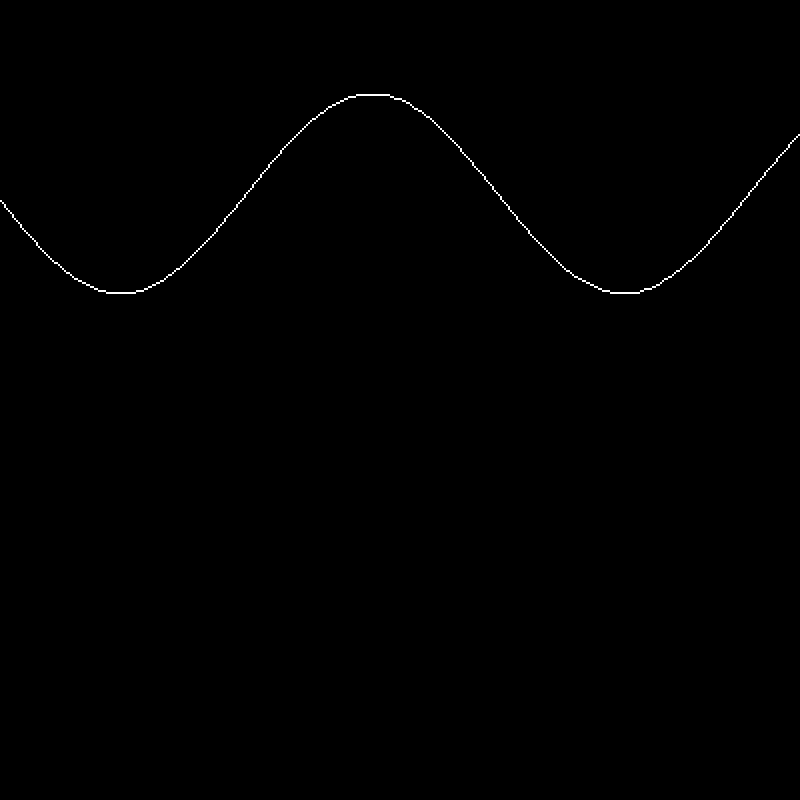
\includegraphics[width=3cm]{images/graph_sine} &
   \vspace{10pt}
   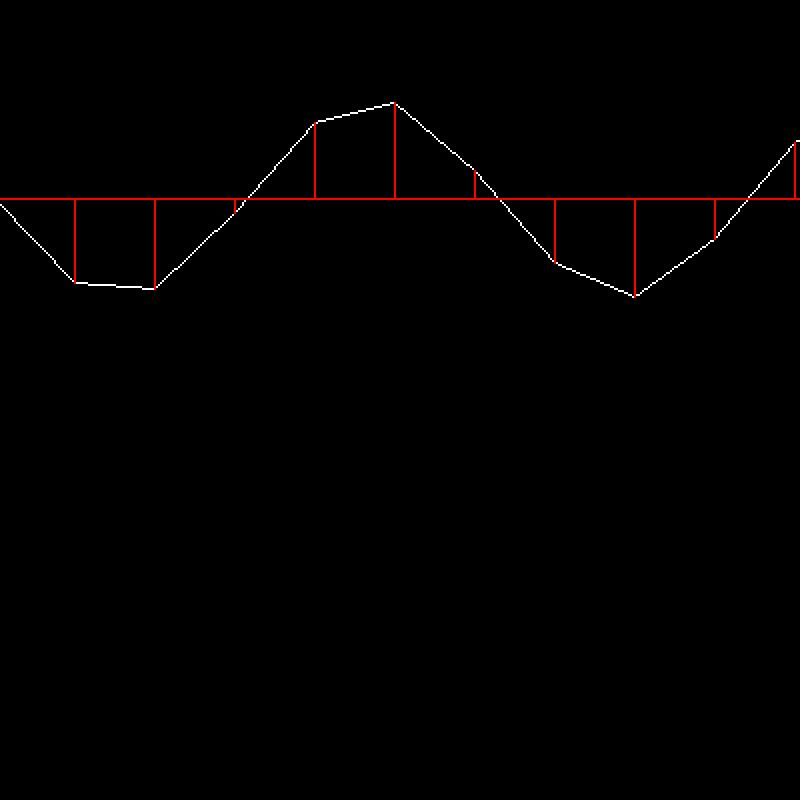
\includegraphics[width=3cm]{images/graph_sine_coarse}\\
   (a)Графика на $y=sin(x)$, нарисувана с 300 отсечки&
   (b)Графика на $y=sin(x)$ с 10 отсечки. Нарисувани са също отсечки между точките от графиката на функцията и абсцисата\\%\hline
   \vspace{10pt}
   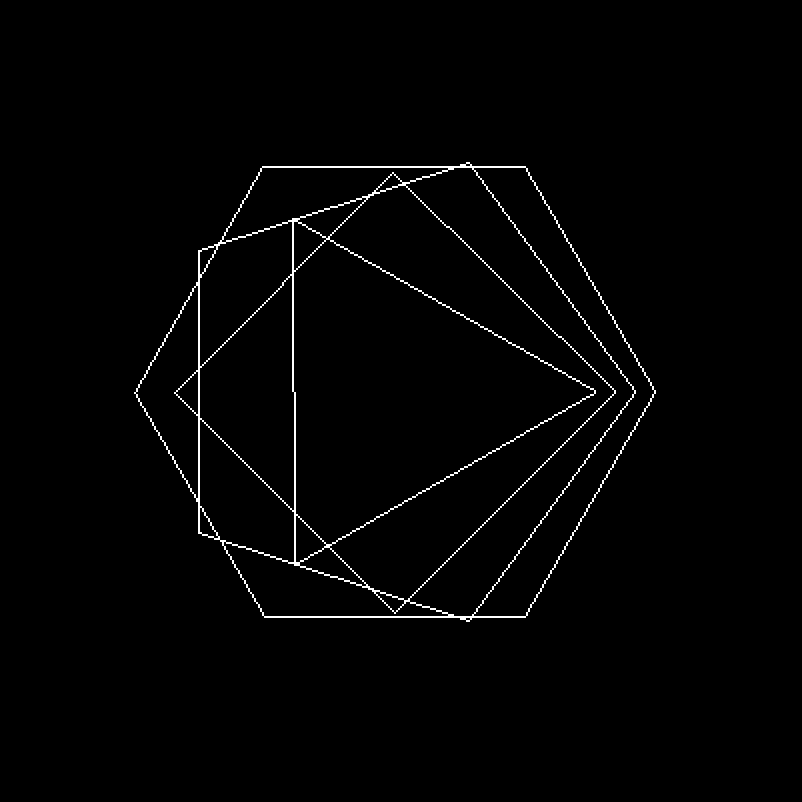
\includegraphics[width=3cm]{images/graph_4_polygons}  &
   \vspace{10pt}
   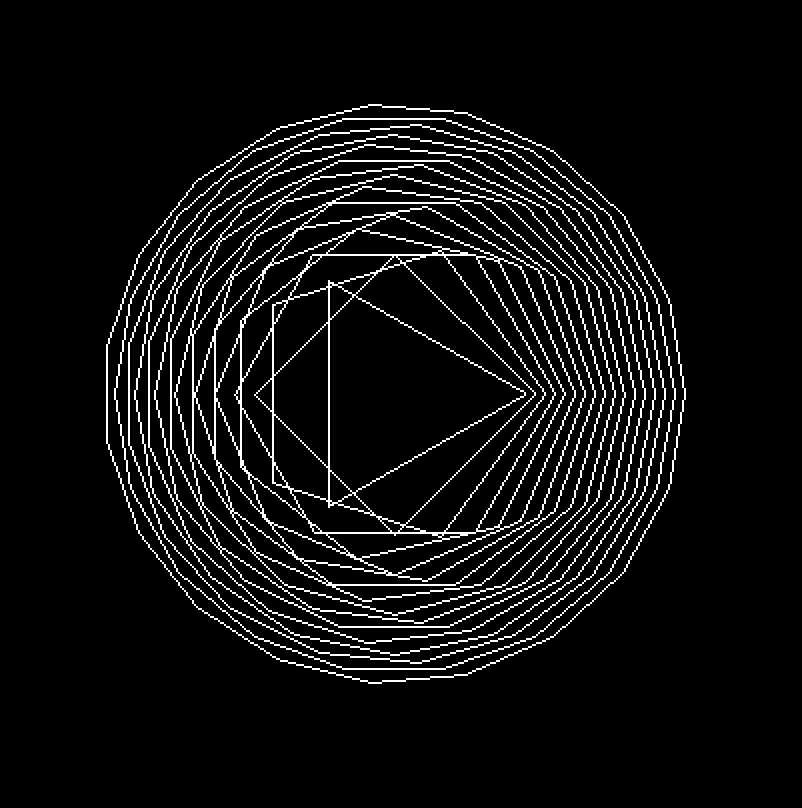
\includegraphics[width=3cm]{images/graph_16_polygons}  \\
   (c)Четири многоъгълника, нарисувани един върху друг с нарастващи радиус и брой върхове
   \vspace{10pt}&
   (d)Шестнадесет многоъгълника, нарисувани един върху друг с нарастващи радиус и брой върхове
   \vspace{10pt}  \\%\hline
   \vspace{10pt}
   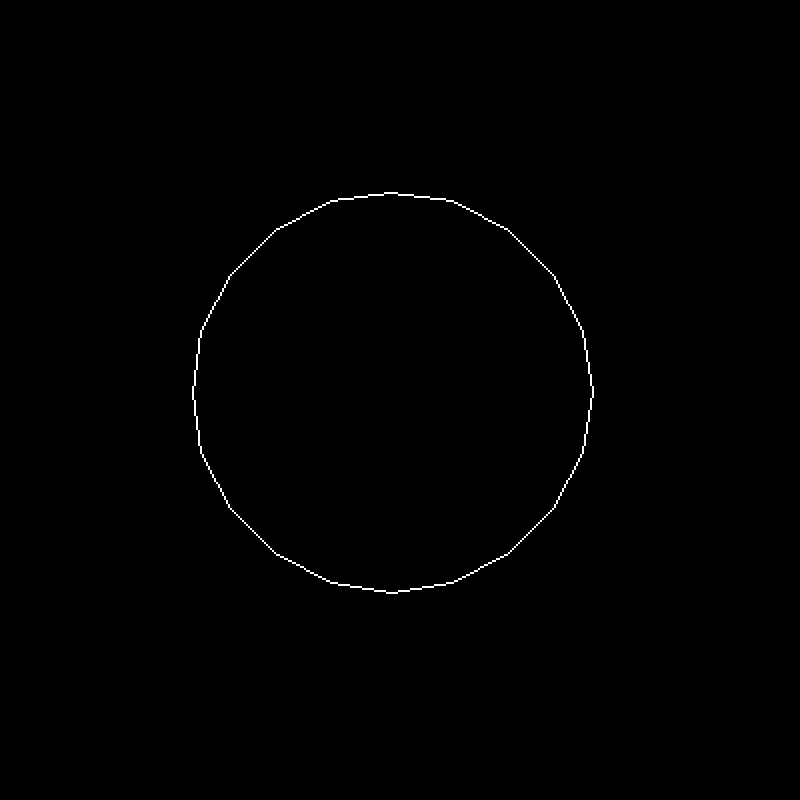
\includegraphics[width=3cm]{images/graph_twentygon}   &
    \\
    (e)Многоъгълник с 20 върха, приближаващ окръжност
   \vspace{10pt} &
   \\\hline
  \end{tabular}
  \end{center}

  \caption{Примерни резултати от решенията на някои задачи}
  \label{fig:drawings}
\end{figure}



\begin{enumerate}[resume]


	\item По дадени екранни координати $(x,y)$ на горния ляв ъгъл на квадрат, дължина на страната $a$ на квадрата и число $n$:

	\begin{itemize}
		\item Да се нарисува квадратна матрица от $n \times $n квадрата със страна $a/n$, изпълваща дадения квдрат.
		\item Квадратите от горното условие да се заменят с тригъгълниците, образувани от пресичането на диагоналите им.
	\end{itemize}

	\item Да се нарисуват програмно следните фигури:

	\begin{itemize}
		\item Равностранен триъгълник
		\item Равностранен шестоъгълник
		\item Равностранен многоъгълник по дадени координати на пресечната точка на симетралите му (център), брой страни $n$ и разстояние от центъра до върховете $r$. При какви стойности на $n$ фигурата наподобява окръжност?
		\item Логаритмична крива
		\item Елипса с център дадени $(x,y)$ и радиуси дадени $r_1$ и $r_2$
	\end{itemize}

  \begin{mdframed}[hidealllines=true,backgroundcolor=gray!20]
    \textbf {Упътване към задачата за чертане на графика на функцията $y=sin(x)$:} Рисуват се отсечки между последователни точки от графиката на функцията, като всяка следваща точка се получава като увеличаваме стойността на аргумента $x$ с числото \code{stepX}. Тъй като $sin(x)\in[-1,1]$, ако директно визуализираме точките на получените по този начин координати $(x,sin(x))$, те ще са ``сгъстени'' около правата $y=0$ и резултатът няма да е добър. Поради това, координатите на получените  точки от кривата се умножават по \code{scaleX} и \code{scaleY} съответно, $(x.scaleX,sin(x).scaleY)$, за да се ``разпъне'' графиката по двете оси. (Вж. Фигура \ref{fig:drawings})\\

    \begin{mdframed}[hidealllines=true,backgroundcolor=lightgray!20]
    \relscale{0.8}
    \begin{verbatim}
    const double //scaleX: коефициент на скалиране по X
                 scaleX = 40.0,
                 //y0: ордината на началната точка
                 y0 = 100,
                 //scaleY: коефициент на скалиране по Y
                 scaleY = 50.0,
                 //stepX: стъпка за нарастване на аргумента
                 stepX = 0.05;
                 //nsegments: брой сегменти от кривата
    const int nsegments = 300;

    for (int i = 0; i < nsegments; i++)
    {
         double x     = scaleX*i*stepX,
                xnext = scaleX*(i+1)*stepX,
                y     = y0+scaleY*sin(stepX*i),
                ynext = y0+scaleY*sin(stepX*(i+1));
         drawLine (x,y,xnext,ynext);
    }
    \end{verbatim}
    \end{mdframed}

    \end{mdframed}

    \begin{mdframed}[hidealllines=true,backgroundcolor=gray!20]

    \textbf {Упътване към задачата за чертане на многоъгълник:} Върховете на мнгоъгълника получаваме, като започнем с точката с координати $(x+radius,y)$ и получаваме всяка следваща точка като ``завъртим'' предишната около $(x,y)$ с $2\pi/n$ радиана, където $n$ е броят на върховете на многоъгълника. Получените по този начин точки се съединияват с отсечки. (Вж. Фигура \ref{fig:drawings} и Фигура \ref{fig:pentagon}.)\\

    \begin{mdframed}[hidealllines=true,backgroundcolor=lightgray!20]
    \relscale{0.8}
    \begin{verbatim}
    /*
    Функция polygon (n,x,y,radius): Рисуване на многоъгълник
    параметър n: брой върхове на многоъгълника
    параметри x,y: координати на центъра на многоъгълника
    параметър radius: разстояние от центъра до върховете
    */
    void polygon (int n, double x, double y, double radius)
    {
      for (int side = 0; side < n; side++)
      {
         drawLine (radius*cos(side*2.0*M_PI/n)+x,
                   radius*sin(side*2.0*M_PI/n)+y,
                   radius*cos((side+1)*2.0*M_PI/n)+x,
                   radius*sin((side+1)*2.0*M_PI/n)+y);
      }
    }
    \end{verbatim}
    \end{mdframed}

    \end{mdframed}

    \begin{figure}
    \centering
    \relscale{0.7}

        \begin{tikzpicture}[auto,>=latex']
        \node [fork, name=center, fill = red] (center) at(4,4){};
        \node [left of = center,node distance = 0.7cm] {\small{$(x_0,y_0)$}};
        %(cos 0, sin 0)
        \node [fork, name=v0] (v0) at(7,4) {};
        \node [right of = v0, node distance=2cm] {\Small{$(x_0+r.cos(0),y_0+r.sin(0))$}};
        %cos 2Pi/5, sin 2pi/5
        \node [fork, name=v1] (v1) at(4.927,6.853) {};
        \node [right of = v1,node distance = 2.8cm] {\Small{$(x_0+r.cos(4\times\frac{2\pi}{5}),y_0+r.sin(4\times\frac{2\pi}{5}))$}};
        %cos 2*2Pi/5, sin 2*2pi/5
        \node [fork, name=v2] (v2) at(1.573,5.763) {};
        %cos 3*2Pi/5, sin 3*2pi/5
        \node [fork, name=v3] (v3) at(1.573,2.237) {};
        %cos 4*2Pi/5, sin 4*2pi/5
        \node [fork, name=v4] (v4) at(4.927,1.147) {};
        \node [right of = v4,node distance = 2.5cm] {\Small{$(x_0+r.cos(\frac{2\pi}{5}),y_0+r.sin(\frac{2\pi}{5}))$}};


        %\draw [->] (test1) -- node []{yes}(end);
        \draw [-] (v0)--(v1);
        \draw [-] (v1)--(v2);
        \draw [-] (v2)--(v3);
        \draw [-] (v3)--(v4);
        \draw [-] (v4)--(v0);
        \draw[densely dashed] (center) -- (v0);
        \draw[densely dashed] (center) -- (v1);
        \draw[densely dashed] (center) -- (v2);
        \draw[densely dashed] (center) -- (v3);
        \draw[densely dashed] (center) -- (v4);
        \draw (4.5,4) arc (0:72:0.5);
        \node [] at (4.7,4.5) {\small{$\frac{2\pi}{5}$}};
        \draw[help lines, densely dotted] (0,0) grid (12,8);
        \draw [->, dashed,semithick](v1) arc (72:432:3);
        \end{tikzpicture}

      \caption{Рисуване на петоъгълник чрез намиране на 5 равноотдалечени точки по окръжността с радиус $r$ и център $(x_0,y_0)$}
      \label{fig:pentagon}
    \end{figure}




	\item Да се нарисува програмно котката Pusheen на Фигура~\ref{fig:pusheen} (вж. \cite{pusheen}).

  \begin{figure}
  \centering
	
\includegraphics[width=10cm]{images/pusheen}
  \caption {Pusheen the cat. Фигурата е от \cite{pusheen}}
  \label{fig:pusheen}
  \end{figure}


  \item(*) \textit{Следната задача илюстрира метода на трапеците (Trapezoidal rule) за приближено изчисление на определени интеграли:}

	Да се нарисуват програмно координатни оси на евклидова коорднинатна система с даден център в екранните координати (x,y). Да приемем, че в програмата е дефинирана функция \code {double f (double x)}, за която знаем, че е дефинирана за всяка стойност на $x$.

	\begin{itemize}
		\item Да се изобрази графиката на фукцията спрямо нарисувана координатна система
		\item Да се приближи чрез трапеци с дадена дължина на основата $\delta$ фигурата, заключена между видимата графика на фигурата и абсцисата
		\item Да се визуализират така получените трапеци
		\item Да се изчисли сумата от лицата на така получените трапеци
		\item Да се експериментра с различни дефиниции на функцията $f$
	\end{itemize}


\end{enumerate}


\section {Цикли, масиви и низове}

\subsection {Цикли \textrm{II}}

Където не е посочено изрично, под ``редица от числа $a_0, a_1, ..., a_{n-1}$'' по-долу се разбира последователност от $n$ числа, въведени от стандартния вход. Задачите да се решат \emph{без} използването на масиви.


\begin{enumerate}[]


		\item Задача 3.1. \cite{sbornik} Да се напише програма, която въвежда редица от n цели числа $(1 \leq n \leq 50)$ и намира и извежда минималното от тях.

		\item Задача 3.2. \cite{sbornik} Да се напише програма, която въвежда редицата от n $(1 \leq n \leq 50)$ цели числа $a_0, a_1, ..., a_{n-1}$ и намира и извежда сумата на тези елементи на редицата, които се явяват удвоени нечетни числа.

		\item Задача 3.3. \cite{sbornik} Да се напише програма, която намира и извежда сумата от положителните и произведението на отрицателните елементи на редицата от реални числа $a_0, a_1, ..., a_{n-1}$ $(1 \leq n \leq 20)$.

		\item Задача 3.7. \cite{sbornik} Да се напише програма, която изяснява има ли в редицата от цели числа $a_0, a_1, ..., a_{n-1}$ $(1 \leq n \leq 100)$ поне два последователни елемента с равни стойности.

		\item Задача 3.8. \cite{sbornik} Да се напише програма, която проверява дали редицата от реални числа $a_0, a_1, ..., a_{n-1}$ $(1 \leq n \leq 100)$ е монотонно растяща.

    \item Задача 3.15. \cite{sbornik} Да се напише програма, която въвежда реланите вектори $a_0, a_1, ..., a_{n-1}$ и $b_0, b_1, ..., b_{n-1}$ $(1 \leq n \leq 100)$,  намира скаларното им произведение  и го извежда на екрана.

		\item Задача 3.10. \cite{sbornik} Да се напише програма, която за дадена числова редица $a_0, a_1, ..., a_{n-1}$ $(1 \leq n \leq 100)$ намира дължината на най-дългата ú ненамаляваща подредица $a_i, a_{i+1}, ..., a_{i+k}$ $(a_i \leq a_{i+1} \leq ... \leq a_{i+k})$.


\end{enumerate}

\subsection {Цикли и низове}
Където не е посочено изрично, под ``редица от символи $s_0, s_1, ..., s_{n-1}$ $(1 \leq n \leq 100)$ $a_0, a_1, ..., a_{n-1}$'' по-долу се разбира символен низ с дължина $n$, въведен от клавиатурата в масив от тип \code{char[255]}.

\begin{enumerate}[resume]


  \item Задача 3.11. \cite{sbornik}	Дадена е редицата от символи $s_0, s_1, ..., s_{n-1}$ $(1 \leq n \leq 100)$. Да се напише програма, която извежда отначало всички символи, които са цифри, след това всички символи, които са малки латински букви и накрая всички останали символи от редицата, запазвайки реда им в редицата.

	\item Задача 3.13. \cite{sbornik} Задача 3.13. Да се напише програма, която определя дали редицата от символи $s_0, s_1, ..., s_{n-1}$ $(1 \leq n \leq 100)$ е симетрична, т.е. четена отляво надясно и отдясно наляво е една и съща.

  \item Да се напише функция, която по два низа намира дължината на най-дългия им общ префикс. \textit{Префикс на низ наричаме подниз със същото начало като дадения. Пример: празният низ и низовете ``a'', ``ab'', и ``abc'' са всички възможни префикси на низа ``abc''. Дължината на най-дългия общ префикс на низовете ``abcde'' и ``abcuwz'' е 3.}

  \item Да се напише функция, която в даден низ замества всички малки латински букви със съответните им големи латински букви.

  \item Да се напише функция \code{reverse(s)}, която превръща даден низ в огледалния му образ. \textit{Например, низът ``abc'' ще се пребразува до ``cba''.}

  \item Да се напише функция, която по даден низ $s$, всички букви в който са латински, извъшва следната манипулация над него: Ако $s$ съдържа повече малки, отколкото големи букви, замества всички големи букви в $s$ с малки. В останалите случаи, всички малки букви се заместват с големи.

	\item Задача 3.26. "Хистограма на символите" \cite{sbornik} Символен низ е съставен единствено от малки латински букви. Да се напише програма, която намира и извежда на екрана броя на срещанията на всяка от буквите на низа.

  \item Да се напише булева функция, която по дадени низове $s_1$ и $s_2$ проверява дали $s_2$ е подниз на $s_1$ (\textit{Например, низът ``uv'' е подниз на низовете ``abuvc'', ``uvz'', ``zuv'' и ``uv'', но не е подниз на низа ``uwv''}.). Функцията да \emph{не} използва вложени цикли.

  \item Задача 3.28. "Търсене на функция" \cite{sbornik} Дадени са два символни низа с еднаква дължина $s_1$ и $s_2$, съставени от малки латински букви. Да се напише програма, която проверява дали съществува функция $f:char \rightarrow char$, изобразяваща $s_1$ в $s_2$, така че $f(s_1[i])$ = $f(s_2[i])$ и $i=1..$дължината на $s_1$ и $s_2$. \textit{Упътване: За да е възможна такава функция, не трябва в $s_1$ да има сивмол, на който съответстват два или повече различни символи в $s_2$. Например, низът ``aba'' може да бъде изобразен в низа ``zwz``, но не и в низа ``zwu''.}

\end{enumerate}


\pagebreak

\subsection {Матрици и вложени цикли}

\begin{enumerate}[resume]

	\item Задача 3.18. \cite{sbornik} Дадени са числовите редици $a_0, a_1, ..., a_{n-1}$ и $b_0, b_1, ..., b_{n-1}$ $(1 \leq n \leq 50)$. Да се напише програма, която въвежда от клавиатурата двете редици и намира броя на равенствата от вида $a_i = b_j$ $(i = 0, ..., n-1, j = 0, ..., n-1)$.

	\item Задача 3.21. \cite{sbornik} Две числови редици си приличат, ако съвпадат множествата от числата, които ги съставят. Да се напише програма, която въвежда числовите редици $a_0, a_1, ..., a_{n-1}$ и $b_0, b_1, ..., b_{n-1}$ $(1 \leq n \leq 50)$ и установява дали си приличат.

	\item Задача 3.29. \cite{sbornik} Дадена е квадратна целочислена матрица A от n-ти ред $(1 \leq n \leq 50)$. Да се напише програма, която намира сумата от нечетните числа под главния диагонал на A (без него).

  \item Задача 3.45. \cite{sbornik} Матрицата А има седлова точка в $a_{i,j}$, ако $a_{i,j}$ е минимален елемент в i-тия ред и максимален елемент в j-тия стълб на A. Да се напише програма, която извежда всички седлови точки на дадена матрица А с размерност $n \times m (1 \leq n \leq 20, 1 \leq m \leq 30)$.

	\item Задача 3.113. (периодичност на масив). \cite{sbornik}	Да се напише програма, която проверява дали в едномерен масив от цели числа съществува период. Например, ако масивът е с елементи 1, 2, 3, 1, 2, 3, 1, 2, 3, 1, периодът е 3. Ако период съществува, да се изведе.

	\item Да се напише програма, която въвежда от клавиатурата матриците от цели числа $A_{N\times M}$ и $B_{M\times N}$ и извежда на екрана резултатът от умножението на двете матрици.


\end{enumerate}

\subsection {Елементарно сортиране на масиви}

\begin{enumerate}[resume]
  \item Да се реализира функция, сортираща масив по метода на мехурчето. При този метод масивът $a[0],..,a[n-1]$ се обхожда от началото към края, като на всяка стъпка се сравняват двойката съседни елементи $a[i]$ и $a[i+1]$. Ако $a[i+1] < a[i]$, местата им се разменят. Този процес се извършва $n$ пъти.
  \item Да се напише функция \code{unsortedness}, която оценява доколко един масив е несортиран като преброява колко от елементите му ``не са на местата си''. Т.е. функцията намира броя на тези елементи $a_i$, които не са $i$-ти по големина в масива. Например, за масива $\{0,2,1\}$ това число е $2$.
  \item Да се напише функция \code{swappable}, която за масива $a[0],..,a[n-1]$ проверява дали има такова число $i(0 < i < n-1)$, че масива $a_i,..,a_n,a_0,..,a_{i-1}$ е стортиран в нарастващ ред. Т.е. може ли масивът да се раздели на две части (незадължително с равна дължина) така, че ако частите се разменят, да се получи нареден масив. Пример за такъв масив е $\{3,4,5,1,2\}$.

\end{enumerate}

\begin{mdframed}[hidealllines=true,backgroundcolor=gray!20]
Функцията \code{std::clock()} от \code{<ctime>} връща в абстрактни единици времето, което е изминало от началото на изпълнение на програмата. Обикновено тази единица за време, наречена ``\code{tick}'', е фиксиран интервал ``реално'' време, който зависи от хардуера на системата и конфирграцията ѝ. Константата \code{CLOCKS\_PER\_SEC} дава броя \code{tick}-ове, които се съдържат в една секунда реално време.

Чрез следния примерен код може да се измери в милисекунди времето за изпълнение на програмния блок, обозначен с ``...''.
\begin{verbatim}
clock_t start = std::clock();
//...
clock_t end = std::clock();

long milliseconds = (double)(end-start)/
                    (CLOCKS_PER_SEC/1000.0);

\end{verbatim}
\end{mdframed}
\begin{mdframed}[hidealllines=true,backgroundcolor=gray!20]
Функцията \code{rand()} от \code{<cstdlib>} генерира редица от псевдо-случайни числа. Всяко последователно изпълнение на функцията генерира следващото число от редицата. За да се осигури, че при всяко изпълнение на програмата ще се генерира различна редица от псевдо-случайни числа, е необходимо да се изпълни функцията \code{srand()} с параметър, който е различен за всяко изпълнение на програмата. Една лесна възможност е да се позлва резултата на функцията \code{time(0)}, която дава текущото време на системния часовник в стандарт \code{epoch time}. Достатъчно е \code{srand()} да се изпълни веднъж за цялото изпълнение на програмата.

Чрез следния примерен код може да се генерира редица от 10 (практически) случайни числа, които са различни при всяко изпълнение на програмата.
\begin{verbatim}
srand (time(0));
for (int i = 0; i < 10; i++)
{
  std::cout << rand () << std::endl;
}
\end{verbatim}
Стойностите на \code{rand()} са в интервала $[0..INT\_MAX]$. Ако е нужно да генерирате стойности в друг интервал, например $[0..N]$, това може да стане по формулата $\frac{rand()}{INT\_MAX}\times N$ (трябва да избегнете целочисленото делене)!
\end{mdframed}

\begin{enumerate}[resume]

  \item Да се измери емпирично времето за изпълнение на алгоритъма за сортиране по метода на мехурчето. Да се начертае графика на зависимостта на времето за изпълнение от големината на масива. Всеки тест да е с наново генериран масив от случайни числа.
  \item Да се въведе матрица от числа $A_{N \times M}$.
  \begin{itemize}
      \item Да се сортира всеки от редовете на матрицата
      \item Да се сортира всяка от колоните на матрицата
  \end{itemize}
  Така получените матрици да се отпечатат на стандартния изход.

\end{enumerate}



\begin{mdframed}[hidealllines=true,backgroundcolor=gray!20]
\code{Bozosort} е случайностен алгоритъм за сортиране на масиви. При този алгоритъм, на всяка стъпка се разменят две случайни числа от масива, след което се проверява дали масивът се е сортирал. Процесът продължава до сортиране на масива.
\end{mdframed}

\begin{enumerate}[resume]

  \item Да се реализира алгоритъма \code{Bozosort}. Да се измери емпирично времето му за изпълнение. \emph{Внимание: тествайте с достатъчно малки масиви, тъй като този алгоритъм е изключително бавен.}

\end{enumerate}

\subsection {Низове II}

\begin{itemize}[resume]

  \item Задача 3.55. \cite{sbornik} Дадена е квадратна таблица $A_{n\times n}$ $(1 \le n \le 30)$ от низове, съдържащи думи с максимална дължина 6. Да се напише програма, която проверява дали изречението, получено след конкатенацията на думите от главния диагонал (започващо от горния ляв ъгъл) съвпада с изречението, получено след конкатенацията на думите от вторичния главен диагонал на A (започващо от долния ляв ъгъл).

  \item Задача 3.56. \cite{sbornik} Дадена е квадратна таблица A от n-ти ред $(1 \le n \le 20)$ от низове, съдържащи думи с максимална дължина 9. Да се напише програма, която намира и извежда на екрана изречението, получено след обхождане на A по спирала в посока на движението на часовниковата стрелка, започвайки от горния ляв ъгъл. Например ако матрицата A има вида:

  $\left( \begin{array}{ccc}
  a & b & c \\
  d & e & f \\
  g & h & i
  \end{array} \right)$

  изречението след обхождането по спирала е: ``abcfihgde''.

  \item Задача 3.57 (Inner Join). \cite{sbornik} Нека са дадени два масива от низове – students и grades с най-много 20 низа във всеки. Низовете в масива students имат вида ``XXXXXX YYYY...'', където ``XXXXXX'' е шестцифрен факултетен номер, а ``YYYY...'' е име с произволна дължина. Низовете в grades имат вида ``XXXXXX YYYY'', където ``XXXXXX'' е шестцифрен факултетен номер, а ``YYYY'' е оценка под формата на число с плаваща запетая. И двата масива са сортирани във възходящ ред по факултетен номер. Възможно е в някой от двата масива да има данни за факултетни номера, за които няма данни в другия. И в двата списъка даден факултетен номер се среща най-много един път. Да се напише програма, която извежда на екрана имената и оценките на тези студенти, за които има информация и в двата списъка, като оценките са увеличени с 1 единица, но са максимум 6.00.

\end{itemize}

\subsection{Инвариант на цикъл и верификация на програми}

\emph{Изложението в тази секция е силно опростена версия на метода на Флойд (Floyd) за верификация на блок схеми, описан в монументалната му статия \cite{floyd}. Редица идеи и задачи са взаимствани от книгата \cite{tpsbornik} на А. Соскова и С. Николова ``Теория на програмите в задачи''. За по-подробно изложение и допълнителни примери и задачи препоръчваме тази книга. Изложението по-долу е нарочно опростено, като на места е жертвана прецизността му.}

\begin{mdframed}[hidealllines=true,backgroundcolor=gray!20]


\bigskip
\textbf{Инвариант на цикъл}
\bigskip


Нека е дадена програма или част от програма, която се се състои от единствен \code{while} цикъл. Нека имаме някакъв набор от работни променливи $v_1,..,v_n$, които се инициализират непосредствено преди \code {while} цикъла. Условието на цикъла зависи изцяло от работните променливи, а тялото на цикъла използва или променя само тях. Приемаме, че програмата не произвежда странични ефекти и не зависи от такива.

Тоест, за програмата знаем, че: (1) не извършва входни и изходни операции, (2) поведението ѝ зависи изцяло от началните стойности на работните променливи $v_1,..,v_n$ и (3) не модифицира никакви други променливи, освен работните. Такава програма можем да изобразим чрез блок схемата на Фигура \ref{fig:1while}.
\end{mdframed}


\begin{figure}
    \begin{tikzpicture}[auto, node distance=1.5cm,>=latex']
    \node [entry, name=start](start){};
    \node [block,name=init, below of = start] (init)
       {Инициализация на\\ $v_0,..,v_n$};
    \node [fork,name=test1fork,below of = init,node distance = 2cm]{};
    \node [condition,name=test1, below of = test1fork,node distance = 3cm] (test1) {Условие \\ $C(v_0,..,v_n)$};
    \node [block,name=inc,right of = test1, node distance = 6.5cm] (inc) {Операции \\$(v_0^i,..,v_n^i) \rightarrow (v_0^{i+1},..,v_n^{i+1})$};
    \node [fork,name=endfork,below of = test1, node distance = 3cm]{};
    \node [entry, name=end, below of = endfork, node distance = 1cm](end){};

    \node [cut, name=cut1, left of = test1fork, node distance = 2cm](cut1){1};
    \node [cut, name=cut2, left of = endfork, node distance = 2cm](cut2){2};

    \draw [->] (start) -- (init);
    \draw [-] (init) -- (test1fork);
    \draw [->] (test1fork) -- (test1);
    \draw [->] (test1) -- node{true} (inc);
    \draw [->] (inc) |- (test1fork);
    \draw [-] (test1) -- node []{false}(endfork);
    \draw [->] (endfork) -- (end);

    \draw [-,dashed] (cut1) -- (test1fork);
    \draw [-,dashed] (cut2) -- (endfork);
    \end{tikzpicture}

  \caption{Блок схема на част от програма с \code{while} цикъл}
  \label{fig:1while}
\end{figure}


\begin{mdframed}[hidealllines=true,backgroundcolor=gray!20]
На фигурата $C(v_1,..,v_n)$ е някакъв логически израз, зависещ само от $v_1,..,v_n$. Да допуснем, че сме ``замразили'' изпълнението на програмата в точката, обозначена с ``1'', точно преди да започне $i$-тото поред ($i\geq 0$) изпълнение на тялото на цикъла, т.е. непосредствено преди да бъдат изпълнени операторите в него за $i$-ти път. В този момент $n$-торката работни променливи $(v_1,..,v_n)$ имат някакви конкретни стойности. Да ги обозначим с $(v_0^{i},..,v_n^{i})$. След изпълнение на всички оператори в тялото на цикъла работните променливи получават някакви нови стойности. Това са точно стойностите $(v_0^{i+1},..,v_n^{i+1})$, които работните променливи ще имат в началото на $i+1$-вата итерация. Това е изобразено на фигурата чрез прехода $(v_0^i,..,v_n^i) \rightarrow (v_0^{i+1},..,v_n^{i+1})$.

Нека приемем, че при някакво конкретно изпълнение на програмата, при конкретни дадени начални стойности на работните променливи  $(v_0^{0},..,v_n^{0})$, тялото на цикъла ще бъде изпълнено точно  $k\geq 0$ пъти, след което условието $C(v_1,..,v_n)$ на цикъла ще се наруши и той ще приключи. Изпълнението на програмата достига точката, обозначена с ``2''. По този начин се получава редицата от $n$-торки $(v_0^{0},..,v_n^{0}),..,(v_0^{k},..,v_n^{k})$, като за всички нейни членове $0\leq i < k$, освен за последния, знаем че е вярно $C(v_0^{i},..,v_n^{i})$, а за последния, $k$-ти член, е вярно обратното --- $\neg C(v_0^{k},..,v_n^{k})$.

Освен свойството $C(v_0^{i},..,v_n^{i})$ (или неговото отрицание), което знаем за всички последователни стойности на работните променливи, можем да въведем още едно свойство $I(v_0^{i},..,v_n^{i})$, наречено ``инвариант на цикъла''. За свойството $I$ искаме да е вярно за всички възможни стойности на работните променливи, дори и за последния член на редицата им. От там идва името ``инвариант'', т.е. факт, което е винаги верен.

Това свойство може да е произволно, например тъждествената истина \code{true} изпълнява условието за инвариант, тъй като е вярна за всички членове на редицата на работните променливи. Инвариантът обаче е най-полезен, когато представя ``смисъла'' на работните променливи, и ако от верността на $\neg C(v_0^{k},..,v_n^{k})\,\&\, I(v_0^{k},..,v_n^{k})$ можем да изведем нещо полезно за ``крайния резултат'' от изпълнението на цикъла, съдържащ се в стойностите $(v_0^{k},..,v_n^{k})$.
\end{mdframed}

\begin{figure}
    \begin{tikzpicture}[auto, node distance=1.5cm,>=latex']
    \node [entry, name=start](start){};
    \node [block,name=init, below of = start, align=left] (init)
       {\code{candidate = 0;}\\\code{current = 1;}};

    \node [fork,name=test1fork,below of = init,node distance = 2cm]{};

    \node [block,name=inc2, right of = test1fork, node distance = 5cm,minimum height=1.5cm]{\code{current++;}};

    \node [condition,name=test1, below of = test1fork,node distance = 3cm] (test1) {\code{current < m}};

    \node [condition, name=test2, right of = test1, node distance = 5cm,font=\tiny] (test2) {\code{A[current]}\\\code{<A[candidate]}};

    \node [block,name=inc,right of = test2, node distance = 5cm, minimum height=1.5cm] (inc) {\code{candidate = current};};

    \node [fork,name=endfork,below of = test1, node distance = 3cm]{};
    \node [entry, name=end, below of = endfork, node distance = 1cm](end){};

    \node [cut, name=cut1, left of = test1fork, node distance = 2cm](cut1){1};
    \node [cut, name=cut2, left of = endfork, node distance = 2cm](cut2){2};

    \draw [->] (start) -- (init);
    \draw [-] (init) -- (test1fork);
    \draw [->] (test1fork) -- (test1);

    \draw [->] (test1) -- node{true} (test2);
    \draw [->] (test2) -- node{true} (inc);

    \draw [->] (inc) |- (inc2);
    \draw [->] (inc2) -- (test1fork);
    \draw [->] (test2) -- node{false} (inc2);


    \draw [-] (test1) -- node []{false}(endfork);
    \draw [->] (endfork) -- (end);

    \draw [-,dashed] (cut1) -- (test1fork);
    \draw [-,dashed] (cut2) -- (endfork);
    \end{tikzpicture}

  \caption{Блок схема на програмата за намиране на най-малък елемент в масив}
  \label{fig:minel}
\end{figure}



\begin{mdframed}[hidealllines=true,backgroundcolor=gray!20]

\bigskip
\textbf{Верификация на програми}
\bigskip

Понятието ``инвариант'' ще илюстрираме чрез едно негово приложение: ``Верификация на програма''. Верификацията на програма е доказателство, че при необходимите начални условия дадена програма изчислява стойност, удовлетворяваща някакво желано свойство. Като пример да разгледаме следната  програма, за която ще се уверим, че намира най-малък елемент на едномерен масив $A$ с $m>0$ елемента $A[0],..,A[m-1]$.


\begin{verbatim}
size_t candidate = 0, current = 1;
while (current < m)
{
  if (A[candidate] < a[current])
  {
    candidate = current;
  }
  current++;
}
\end{verbatim}
Можем да приложим метода на инварианта, за да докажем строго, че когато цикълът приключи, то елементът $A[candidate]$ е гарантирано по-малък или равен на всички останали елементи на масива.
Като първа стъпка, за улеснение изобразяваме програмата като блок схемата на Фигура \ref{fig:minel}.


Работните променливи на програмата, освен масива $A$, са целочислените променливи \code{candidate} и \code{current}. Какъв е смисълът на тези променливи? Веднага се вижда, че \code{current} е просто брояч --- служи за обхождане на елементите на масива последователно от $A[0]$ до $A[m-1]$, като на всяка итерация от цикъла се разглежда стойността на $A[current]$.

Интуитивно се вижда, че \code{candidate} е намереният най-малък елемент на масива до текущия момент от обхождането. Тоест, можем да се надяваме, че ако сме разгледали първите $i$ елемента на масива, то правилно сме определили, че най-малкият от тях е $A[current]$.

Тези размишления може да запишем чрез инварианта:

$I ::= A[candidate]=min(A[0],..,A[current-1])$.

Този инвариант очевидно е верен в началото на изпълнението на програмата, когато $current=1$, а $candidate=0$. Как да се уверим, че инвариантът е валиден за всички стойности, през които преминават работните променливи?

Нека допуснем, че инвариантът е верен за някаква стъпка $i$ от изпълнението на цикъла. Тоест, допускаме $I(candidate^i, current^i)$, или $A[candidate^i]=min(A[0],..,A[current^i-1])$.

На итерация $i+1$ имаме  и $current^{i+1}=current^{i}+1$, и следователно трябва да покажем, че $A[candidate^{i+1}]=min(A[0],..,A[current^{i+1}-1])$.

След навлизане в тялото на цикъла, имаме две възможности:
\begin{enumerate}[label=\arabic*)]
  \item $A[current^i]\geq A[candidate^i]$. От допускането следва, че добавянето на $A[current^i]$ към $min(A[0],..,A[current^i-1])$ не променя стойността на минимума, или $min(A[0],..,A[current^i-1])=min(A[0],..,A[current^i-1],A[current^i])$. От тук директно се вижда, че инвариантът е верен за итерация $i+1$.
  \item $A[current^i] < A[candidate^i$]. Тъй като по допускане $A[candidate^i] = min(A[0], .., A[current^i-1])$, от тук следва, че $A[current^i] < min(A[0], .., A[current^i-1])$, следователно

   $A[current^i] = min(A[0], .., A[current^i-1], A[current^i])$.

   Но след присвояването имаме $candidate^{i+1} = current^i$, от където $A[candidate^{i+1}] = min(A[0],..,A[current^i])$. Но $current^i = current^{i+1}-1$, от където получаваме верността на $I$ за итерация $i+1$: $A[candidate^{i+1}] = min(A[0], .., A[current^{i+1}-1])$.

\end{enumerate}
  Доказателството протича по индукция. Уверяваме се, че инвариантът е верен за цялата редица от стойности на \code{candidate} и \code{current}.

  Какво се случва в края на цикъла, когато имаме $\neg(current<m)$? Тъй като числата са цели, а \code{current} се увеличава само с единица, можем да заключим, че $current=m$. Замествайки това равенство в инварианта, получаваме твърдението

  $A[candidate] = min(A[0], .., A[m-1])$.

  Тоест, намерили сме минималния елемент на масива.
\end{mdframed}

\begin{enumerate}[resume]
  \item Да се докаже строго, че за следната функция е вярно $pow(x,y)=x^y$:
  \begin{enumerate}[label=\alph*)]%[a)] % a), b), c), ...

    \item
\begin{verbatim}
unsigned int pow (unsigned int x, usnigned int y)
{
  unsigned int p = 1, i = 0;
  while (i < y)
  {
    p *= x;
    i++;
  }
  return p;
}
\end{verbatim}
    \item
\begin{verbatim}
unsigned int pow (unsigned int x, usnigned int y)
{
  unsigned int p = 1;
  while (y > 0)
  {
    p *= x;
    y--;
  }
  return p;
}
\end{verbatim}
      \item
\begin{verbatim}
unsigned int pow (unsigned int x, usnigned int y)
{
  unsigned int z = x, t = y, p = 1;
  while (t > 0)
  {
    if (t%2 == 0)
    {
      z *= z;
      t /= 2;
    }else{
      t = t - 1;
      p *= z;
    }
  }
  return p;
}
\end{verbatim}
  \end{enumerate}

  \item Да се докаже строго, че за следната функция е вярно $sqrt(n)=[\sqrt{n}]$.

\begin{verbatim}
unsigned int sqrt (unsigned int n)
{
  unsigned int x = 0, y = 1, s = 1;
  while (s <= n)
  {
    x++;
    y += 2;
    s += y;
  }
  return x;
}
\end{verbatim}

\item Да се напише програма, която проверява дали дадени два масива $A$ и $B$ с еднакъв брой елементи $m$ са еднакви, т.е. съдържат същите елементи в същия ред. Да се докаже строго, че програмата работи правилно.

\item Да се докаже, че следната функция връща истина тогава и само тогава, когато масивът \code{A} с \code{n} елемента съдържа елемента \code{x}.

\begin{verbatim}
bool member (int A[], size_t n, int x)
{
  size_t i = 0;
  while (i < n && A[i] != x)
  {
    i++;
  }
  return i < n;
}
\end{verbatim}

\item Да се напише програма, която проверява дали даден масив $A$ с $m$ елемента е сортиран, т.е. дали елементите му са наредени в нарастващ ред. Да се докаже строго, че програмата работи правилно.

\end{enumerate}

\begin{mdframed}[hidealllines=true,backgroundcolor=gray!20]
Съществуват редица съвременни методи за верификация на програми. Пълната версия на метода, използван по-горе, се нарича ``логика на Флойд-Хоар'' (Floyd–Hoare logic) и е само един представител на този клас методи.

Също така, в компютърните науки има направление, наречено ``Синтез на програми'' (Program refinement). При синтеза на програми се решава обратната задача: по спецификация на входа и изхода да се генерира програма, която удовлетворява спецификацията.

Препоръчваме на любознателния читател да се запознае с логиката на Floyd–Hoare и методите за синтез на програми.
\end{mdframed}

\pagebreak

\section{Указатели и програмен стек}

\subsection {Предаване на масиви и указатели като параметри на функции}
\begin{enumerate}
  \item Да се дефинира функция, която получава като параметри два масива с еднакъв брой елементи. Функцията да разменя съответните елементи на масивите ($a[i] \leftrightarrow b[i]$).
  \item Да се дефинира функция \texttt{swap([подходящ тип] a,[подходящ тип] b)}, която разменя стойностите на две целочислени променливи, предадени на функцията чрез a и b.
\end{enumerate}

\subsection {Масиви от указатели}
\begin{enumerate}[resume]
  \item Да се напише булева функция \code{bool duplicates (long *ponters[])}, която получава като параметър масив \code{pointers} от указатели към целочислени променливи. Функцията да проверява дали поне две от съответните променливи имат еднакви стойности.
  \item Да се дефинира функцията  \texttt{bool commonel (int *arrays[],int npointers, int arrlengths[])}. Масивът \texttt{arrays} съдъръжа \texttt{npointers} на брой указатели към масиви от цели числа. \texttt{i}-тият масив има големина \texttt{arrlengths[i]}. Функцията да връща истина, ако има поне едно число $x$, което е елемент на всички масиви.
  \item Да се дефинира функцията \texttt{bool subarrays (int *arrays[],int npointers, int arrlengths[])}. Масивът \texttt{arrays} съдъръжа \texttt{npointers} на брой указатели към масиви от цели числа. \texttt{i}-тият масив има големина \texttt{arrlengths[i]}. Функцията да връща истина, ако поне един от масивите е подмасив на друг масив. Масивът $a$ наричаме подмасив на $b$, ако заетата от $a$ памет е част от заетата от $b$ памет. Да се напишат подходящи тестове за функцията.
\end{enumerate}

\subsection {Програмен стек}
\begin{enumerate}[resume]
  \item Да се дефинира рекурсивна функция \code{double sum(size\_t n)}, която въвежда $n$ числа от стандартния вход връща сумата им. \emph{Да не се използват оператори за цикъл!}

  \item Да се дефинира рекурсивна функция \code{reverse(n)}, която въвежда $n$ числа от стандартния вход и ги извежда в обратен ред. \emph{Да не се използват масиви. Да се използва програмния стек чрез рекурсия.}

  \item Да се дефинира функция \code{void getmax (long *pmax, size\_t n)}, която въвежда $n$ числа от стандартния вход и записва максималното от тях в променливата, сочена от указателя \code{pmax}.

  Пример: Следната програма ще изведе най-малкото от 5 въведени от стандартния вход числа.
  \begin{verbatim}
  int main ()
  {
    long max = -1;
    getmax (&max,5);
    std::cout << max;

    return 0;
  }
  \end{verbatim}
  \emph{Функцията да се реализира по два начина: чрез цикъл и чрез използване на рекурсия без оператори за цикъл.}
\end{enumerate}

\pagebreak

\section {Рекурсия}
\subsection {Прости рекурсивни функции}

\begin{enumerate}

	\item Задача 5.2.\cite{sbornik} Да се дефинира рекурсивна функция за намиране на стойността на полинома на Ермит $Hn(x)$ (x е реална променлива, а n неотрицателна цяла променлива), дефиниран по следния начин:

	$H_0(x)=1$

	$H_1(x)=2x$

	$H_n(x)=2xH_{n-1}(x)+2(n-1)H_{n-2}(x), n>1$


	\item Задача 5.3.\cite{sbornik} Произведението на две положителни цели числа може да се дефинира по
следния начин:

	$mult (m,n) = m$, ако n = 1

	$mult (m,n) = m + mult (m,n-1)$, иначе.

	Да се дефинира рекурсивна функция, която намира произведението на две положителни цели числа по описания по-горе начин.

	\item Задача 5.5.\cite{sbornik} Да се дефинира функция, която намира най-големия общ делител на две неотрицателни цели числа, поне едното от които е различно от 0.

	\item Задача 5.7.\cite{sbornik} Дадени са естествените числа n и k $(n \ge 1, k > 1)$. Да се дефинира рекурсивна функция, която намира произведението на естествените числа от 1 до n със стъпка k.

	\item Задача 5.10.\cite{sbornik} Дадено е неотрицателно цяло число n в десетична бройна система. Да се дефинира рекурсивна функция, която намира сумата от цифрите на n в бройна система с основа k $(k > 1)$.

	\item Задача 5.11.\cite{sbornik} Да се дефинира рекурсивна функция, която установява дали в записа на неотрицателното цяло числo n, записано в десетична бройна система, се съдържа цифрата k.

	\item Задача 5.19.\cite{sbornik} Да се дефинира рекурсивна функция, която проверява дали дадено положително цяло число е елемент на редицата на Фибоначи.

	\item Задача 5.28.\cite{sbornik} Да се дефинира рекурсивна функция, която намира максималния елемент на редицата от цели числа $a_0, a_1, a_2, ..., a_{n-1}$, където $n \ge 1$.

	Забележка: Редицата е представена като масив.

	\item Задача 5.31.\cite{sbornik} Да се напише функция

	\texttt{void insertSorted (long x, long arr[], long n)},

	която включва цялото число \texttt{x} число в сортирана във възходящ ред редица от цели числа \texttt{arr}, в която има записани \texttt{n} елемента. Вмъкването да запазва наредбата на елементите. Предлолага се, че за редицата е заделена достатъчно памер за допълване с още едно число.

	\item Задача 5.34.\cite{sbornik} Да се дефинира рекурсивна функция, която сравнява лексикографски два символни низа.
\end{enumerate}

\subsection{Търсене с пълно изчерпване}


\begin{figure}
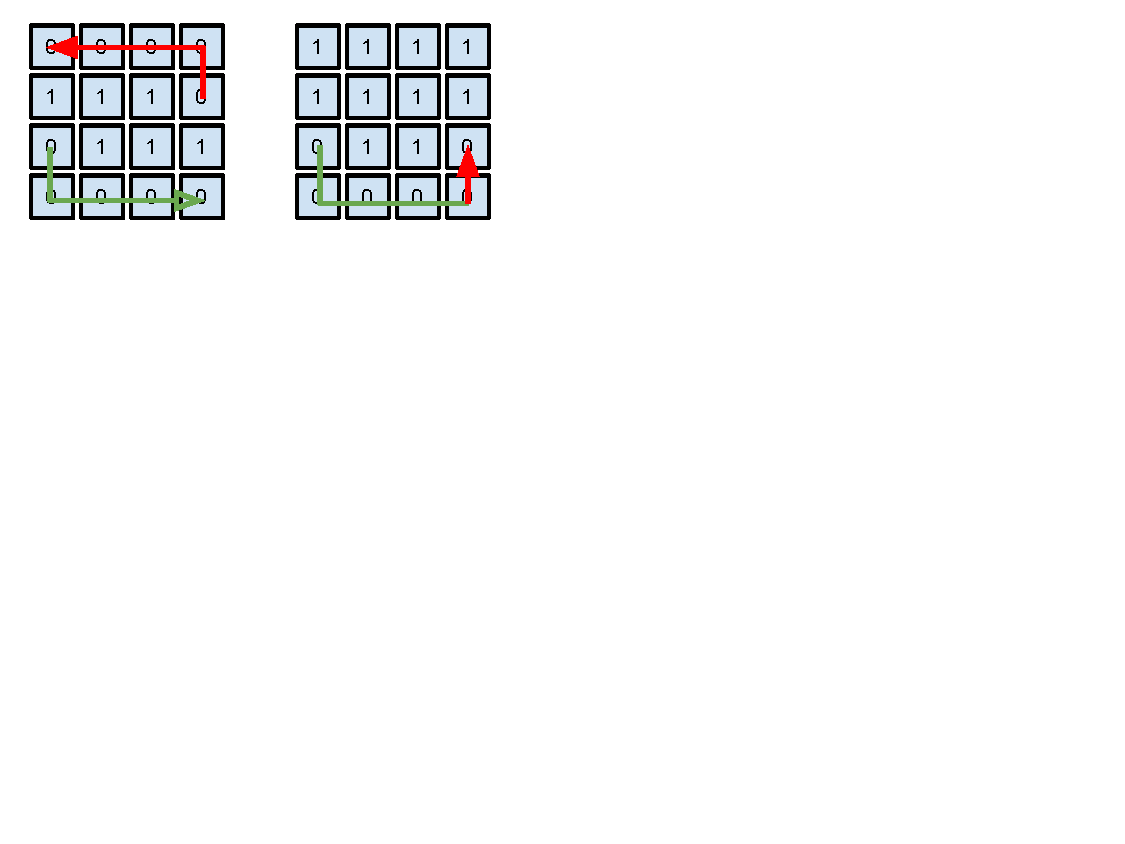
\includegraphics[width=15cm]{images/path1}
\vspace{-200px}
\caption{Примерени лабиринти}
\label{fig:samplelab}
\end{figure}


\begin{enumerate}[resume]

	\item \label{zad:labds} Нека е дадена квадратна матрица от цели числа $N \times N$, представяща ``лабиринт''. Елементи на матрицата със стойност $0$ смятаме за ``проходими'', а всички останали - за ``непроходими''. Път в лабиринта наричаме всяка последователност от проходими елементи на матрицата, които са съседни вертикално или хоризонтално, такава че (1) никой елемент от последователноста не е последван директно от предшественика си (забранено е ``връщането назад'') и (2) най-много един елемент на последователноста се среща в нея повече от веднъж (има най-много един ``цикъл'').

	Да се дефинира функция \texttt{bool downstairs (int sx, int sy, int tx, int ty)}, която проверява дали съществува път от елемента $(sx,sy)$ до елемента $(tx,ty)$, такъв, че всеки следващ елемент от пътя е или вдясно, или под предишния. Такъв път да наричаме ``низходящ''.

	Пример: На Фигура \ref{fig:samplelab}(а) такъв път съществува от елемента $(0,2)$ до елемента $(3,3)$, но не и от $(3,1)$ до $(0,0)$.

	\item При условията на дефинициите от предишната задача, да се дефинира функция \texttt{bool connected()}, която проверява дали от всеки елемент на матрицата $(sx,sy)$ до всеки елемент на матрицата  $(tx,ty)$, такива, че $sx \leq tx$ и $sy \leq ty$, съществува низходящ път.

	Пример: За лабиринта от Фигура \ref{fig:samplelab}(а) условието е изпълнено, но не и за лабиринта отФигура \ref{fig:samplelab}(б).


	\item Да се напише програма, която по въведени от клавиатурата $4 \le n \le 8$ и $0 \le k \le n$ намира извежда на екрана всички възможни конфигурации на абстрактна шахматна дъска с размери $n \times n$ с разположени на нея $k$ коня така, че никоя фигура не е поставена на поле, което се ``бие'' от друга фигура според съответните шахматни правила.

	Пример за отпечатана конфигурация с $n=5, k=2$:
	\begin{verbatim}
	_ _ _ _ _
	_ _ H _ _
	_ _ _ _ _
	_ _ _ _ H
	_ _ _ _ _

	\end{verbatim}


	\item При условията на задача \ref{zad:labds} да се напише функция

	\texttt{int minDistance (int sx, int sy, int tx, int ty)},

	която по въведени от клавиатурата координати на елементи $s=(sx,sy)$ и $t=(tx,ty)$ намира \textit {дължината} на най-краткия път между $s$ и $t$. Обърнете внимание, че се иска \textit{път}, а не просто низходящ път.

	\item

	При условията на задача \ref{zad:labds} да се напише функция, която по въведени от клавиатурата координати на елементи $s=(sx,sy)$ и $t=(tx,ty)$ намира и отпечатва на екрана елементите, от които се състои най-краткия път между $s$ и $t$. Обърнете внимание, че се иска \textit{път}, а не просто низходящ път.


	\item Пъзел на Синди\cite{cindy}.

	Дадена е игрова дъска като на фигура 2, която се състои от $n$ черни и $n$ бели фигури. Фигурите могат да бъдат разположени на $2n+1$ различни позиции. Играта започва с разполагане на всички черни фигури вляво, а всички бели - вдясно на дъската.

	Черните фигури могат да се местят само надясно, а белите - само наляво. На всеки ход важат следните правила:


	\begin{itemize}
		\item всяка фигура се мести само с по една позиция, ако съответната позиция не е заета;
		\item ако позицията е заета, фигурата $X$ може да прескочи точно една фигура $Y$ от противоположния цвят, ако позицията след $Y$ e свободна.
	\end{itemize}

	Да се напише програма, която по въведено число $n$ отпечатва на екрана инструкции за игра така, че в края на играта всички бели фигури да са вляво на дъската, а всички черни - вдясно. Инструкциите да са от следния вид:

	\begin{verbatim}
		...
		Преместете черна фигура фигура от позиция 1 на позиция 2.
		Преместете бяла фигура от позиция 5 на позиция 3.
		...
	\end{verbatim}

	Допустимо е инструкциите да бъдат отпечатани в обратен ред.

	\Bigskip

	\begin{mdframed}[hidealllines=true,backgroundcolor=gray!20]

		На следните фигури е даден пример за игра:

		\begin{flushleft}
		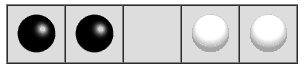
\includegraphics[width=5cm]{images/step0}

		\relscale{0.8}
		1. Начална конфигурация.
		\end{flushleft}


		\begin{flushleft}
		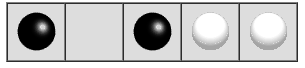
\includegraphics[width=5cm]{images/step1}

		\relscale{0.8}
		2. Преместване на черна фигура с един ход надясно.
		\end{flushleft}

		\begin{flushleft}
		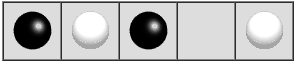
\includegraphics[width=5cm]{images/step2}

		\relscale{0.8}
		3. Преместване на бяла фигура с прескачане.
		\end{flushleft}

		\begin{flushleft}
		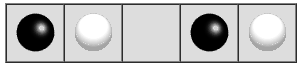
\includegraphics[width=5cm]{images/step3}

		\relscale{0.8}
		4. Преместване на черна фигура с един ход надясно.
		\end{flushleft}

		\begin{flushleft}
		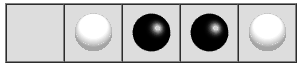
\includegraphics[width=5cm]{images/step4}

		\relscale{0.8}
		5. Преместване на черна фигура чрез прескачане
		\end{flushleft}

		След ход 5 конфигурацията на играта е безперспективна.

	\end{mdframed}

\end{enumerate}


\pagebreak


\begin{thebibliography}{99}

\bibitem{sbornik}	Магдалина Тодорова, Петър Армянов, Дафина Петкова, Калин Георгиев, ``Сборник от задачи по програмиране на C++. Първа част. Увод в програмирането''
\bibitem{tprog} А. Дичев, И. Сосков, ``Теория на програмите'', Издателство на СУ, София, 1998
\bibitem{pusheen} Wikihow, How to Draw Pusheen the Cat, https://www.wikihow.com/Draw-Pusheen-the-Cat
\bibitem{floyd} R. W. Floyd. ``Assigning meanings to programs.'' Proceedings of the American Mathematical Society, Symposia on Applied Mathematics. Vol. 19, pp. 19–31. 1967.
\bibitem{tpsbornik}	Александра Соскова, Стела Николова, ``Теория на програмите в задачи'', Софтех, 2003
\bibitem{cindy}	David Matuszek, ``Backtracking'', https://www.cis.upenn.edu/~matuszek/cit594-2012/Pages/backtracking.html.

\end{thebibliography}

\end{document}
